\chapter{जल और छोटे जैव-अणु}\label{ch:b1:water-small-molecules}

एक घन माइक्रोमीटर के किसी जीवाणु में कोई बीस अरब जल-अणु हैं और बाक़ी हर
चीज़ के कुछ करोड़। \omterm{def:b1:water-small-molecules:water}{जल} \omterm{def:b1:cell-unit-of-life:cell}{कोशिका} की पृष्ठभूमि नहीं, उसका माध्यम है: वह आयन
और शर्कराएँ घोलता है, प्रोटीनों तथा झिल्लियों के तैलीय भाग छिपाता है, वह
अम्लता तय करता है जिस पर हर एंजाइम निर्भर है, और उपापचय की आधी
अभिक्रियाओं में वह अभिकारक या उत्पाद है। यह अध्याय \omterm{def:b1:water-small-molecules:water}{जल} और उन दुर्बल बंधों
का वर्णन करता है जिन्हें वह बनाता और तोड़ता है, अम्लों, क्षारकों तथा
\omterm{def:b1:water-small-molecules:buffer}{बफ़रों} का अंकगणित, वे छोटे कार्बनिक अणु जिनसे अगले चार अध्यायों के
वृहदणु बनते हैं, और ऊर्जा की वह मुद्रा --- \omterm{def:b1:water-small-molecules:atp}{ATP} --- जिसमें \omterm{def:b1:cell-unit-of-life:cell}{कोशिका} उन्हें
बनाने की क़ीमत चुकाती है।

\section{जल}

\begin{definition}[जल-अणु]\label{def:b1:water-small-molecules:water}
\index{जल}
जल, $\mathrm{H_2O}$, एक मुड़ा हुआ अणु है (H--O--H कोण
$104.5^\circ$ है) जिसमें ऑक्सीजन साझा इलेक्ट्रॉनों को अपनी ओर खींचता है:
वह \emph{ध्रुवीय}\index{ध्रुवीय अणु} है, और ऑक्सीजन पर आंशिक ऋण आवेश तथा
हाइड्रोजनों पर आंशिक धन आवेश रखता है। हर अणु चार तक \emph{हाइड्रोजन
बंध}\index{हाइड्रोजन बंध} बना सकता है --- यानी किसी विद्युत-ऋणात्मक
परमाणु (O, N) से बँधे किसी हाइड्रोजन और किसी दूसरे विद्युत-ऋणात्मक परमाणु
के एकाकी युग्म के बीच का स्थिरवैद्युत आकर्षण --- दो अपने हाइड्रोजनों से
और दो अपने ऑक्सीजन से। द्रव जल ऐसे ही बंधों का एक जाल है, जिनमें से हर
एक कुछ पिकोसेकंड टिकता है।
\end{definition}

\begin{omfigure}
\begin{tikzpicture}[font=\small, line cap=round,
  O/.style={circle, draw, thick, fill=omThm!30, minimum size=8mm, inner sep=0pt},
  H/.style={circle, draw, thick, fill=gray!15, minimum size=5.5mm, inner sep=0pt}]
  % central water molecule
  \node[O] (O) at (0,0) {O};
  \node[H] (H1) at (-0.8,-0.7) {H};
  \node[H] (H2) at (0.8,-0.7) {H};
  \draw[thick] (O) -- (H1); \draw[thick] (O) -- (H2);
  \node[font=\scriptsize, omThm] at (0,0.62) {$\delta^-$};
  \node[font=\scriptsize] at (-1.4,-0.55) {$\delta^+$};
  \node[font=\scriptsize] at (1.4,-0.55) {$\delta^+$};
  % lower-left neighbour (accepts an H bond from H1)
  \node[O] (O2) at (-2.1,-2.3) {O};
  \node[H] (H2a) at (-3.05,-2.55) {H};
  \node[H] (H2b) at (-1.75,-3.3) {H};
  \draw[thick] (O2) -- (H2a); \draw[thick] (O2) -- (H2b);
  \draw[dashed, thick, omDef] (H1) -- (O2);
  % lower-right neighbour
  \node[O] (O3) at (2.1,-2.3) {O};
  \node[H] (H3a) at (3.05,-2.55) {H};
  \node[H] (H3b) at (1.75,-3.3) {H};
  \draw[thick] (O3) -- (H3a); \draw[thick] (O3) -- (H3b);
  \draw[dashed, thick, omDef] (H2) -- (O3);
  % upper-left neighbour (donates an H bond to O)
  \node[H] (H4) at (-1.1,1.55) {H};
  \node[O] (O4) at (-2.0,2.25) {O};
  \node[H] (H4b) at (-2.95,2.6) {H};
  \draw[thick] (O4) -- (H4); \draw[thick] (O4) -- (H4b);
  \draw[dashed, thick, omDef] (H4) -- (O);
  % upper-right neighbour
  \node[H] (H5) at (1.1,1.55) {H};
  \node[O] (O5) at (2.0,2.25) {O};
  \node[H] (H5b) at (2.95,2.6) {H};
  \draw[thick] (O5) -- (H5); \draw[thick] (O5) -- (H5b);
  \draw[dashed, thick, omDef] (H5) -- (O);
  \node[anchor=west, align=left, font=\footnotesize] at (4.0,1.0) {बिंदुदार: हाइड्रोजन बंध\\ (\qty{0.18}{nm}, हर एक लगभग \qty{20}{kJ/mol})\\ ठोस: सहसंयोजी O--H बंध\\ (\qty{0.096}{nm}, \qty{460}{kJ/mol})};
  \node[anchor=west, align=left, font=\footnotesize] at (4.0,-1.3) {हर अणु दो हाइड्रोजन बंध\\ देता है और दो लेता है:\\ एक चतुष्फलकी जाल};
\end{tikzpicture}

{\small एक जल-अणु (H--O--H कोण $104.5^\circ$) और उसके चार
हाइड्रोजन-बद्ध पड़ोसी। \omterm{def:b1:water-small-molecules:water}{ध्रुवीय} मुड़ा हुआ अणु अपने हाइड्रोजनों से दो \omterm{def:b1:water-small-molecules:water}{हाइड्रोजन बंध} देता है
और अपने ऑक्सीजन पर दो लेता है; और उनका बनाया जाल \omterm{def:b1:water-small-molecules:water}{जल} को उसका संसंजन,
उसकी ऊष्माधारिता और विलायक के रूप में उसकी शक्ति देता है।}
\end{omfigure}

\begin{proposition}[जल के वे गुण जो जीवन के लिए मायने रखते हैं]\label{prop:b1:water-small-molecules:properties}
हाइड्रोजन-बंध का जाल \omterm{def:b1:water-small-molecules:water}{जल} के असाधारण गुण समझा देता है:
\begin{itemize}
  \item ऊँचा \emph{संसंजन} और पृष्ठ तनाव (\qty{72}{mN/m}): जल-स्तंभ
        बिना टूटे किसी पेड़ पर ऊपर खींचे जा सकते हैं
        (\cref{ch:b1:plant-transport}); कीट तालाबों पर चलते हैं;
  \item ऊँची \emph{ऊष्माधारिता} (\qty{4.18}{kJ.kg^{-1}.K^{-1}}) और
        वाष्पन ऊष्मा (\qty{2.4}{kJ/g}): \omterm{def:b1:organism-environment:organism}{जीवों} का और जल-निकायों का ताप
        धीरे बदलता है, और एक ग्राम पसीने का वाष्पन \qty{2.4}{kJ} हटा
        देता है;
  \item \emph{द्रव से कम सघन ठोस}: बर्फ़ तैरती है, और झीलें ऊपर से
        नीचे की ओर जमती हैं, जिससे नीचे द्रव \omterm{def:b1:water-small-molecules:water}{जल} बचा रहता है;
  \item आयनों और \omterm{def:b1:water-small-molecules:water}{ध्रुवीय अणुओं} के लिए उत्कृष्ट \emph{विलायक}, जिन्हें वह
        अनुस्थापित खोलों से घेर लेता है (\emph{जलयोजन}), और अध्रुवीय
        अणुओं के लिए घटिया विलायक, जिन्हें वह आपस में सटा देता है
        (\emph{जलविरागी प्रभाव}\index{जलविरागी प्रभाव})।
\end{itemize}
\end{proposition}
\begin{proof}[आंशिक उपपत्ति]
संसंजन और पृष्ठ तनाव उन अणुओं को अलग करने का कार्य मापते हैं जिनमें से हर
एक लगभग \qty{20}{kJ/mol} के चार बंधों से थमा है। \omterm{def:b1:water-small-molecules:water}{जल} गरम करने में अणुओं
को हिलाने के साथ-साथ बंध भी तोड़ने पड़ते हैं, इसलिए इतनी ऊष्माधारिता; और
उसे वाष्पित करने में सारे बंध तोड़ने पड़ते हैं। बर्फ़ हर अणु को चार
बंधों की किसी खुली चतुष्फलकी जालक में रखती है, जो अव्यवस्थित द्रव से अधिक
आयतन घेरती है, क्योंकि द्रव में अणु अधिक पास-पास जमते हैं। आयन और
\omterm{def:b1:water-small-molecules:water}{ध्रुवीय} समूह \omterm{def:b1:water-small-molecules:water}{जल} से बने \omterm{def:b1:water-small-molecules:water}{हाइड्रोजन बंधों} से स्थायी होते हैं; कोई अध्रुवीय
अणु वे बंध नहीं बना सकता, और उसके चारों ओर के \omterm{def:b1:water-small-molecules:water}{जल} को स्वयं को किसी पिंजरे
में सजाना पड़ता है, जिसकी क़ीमत एंट्रॉपी में चुकानी पड़ती है और जो तब घट
जाती है जब अध्रुवीय अणु गुच्छा बनाकर एक ही पिंजरा साझा कर लें।
\end{proof}

\begin{omfigure}
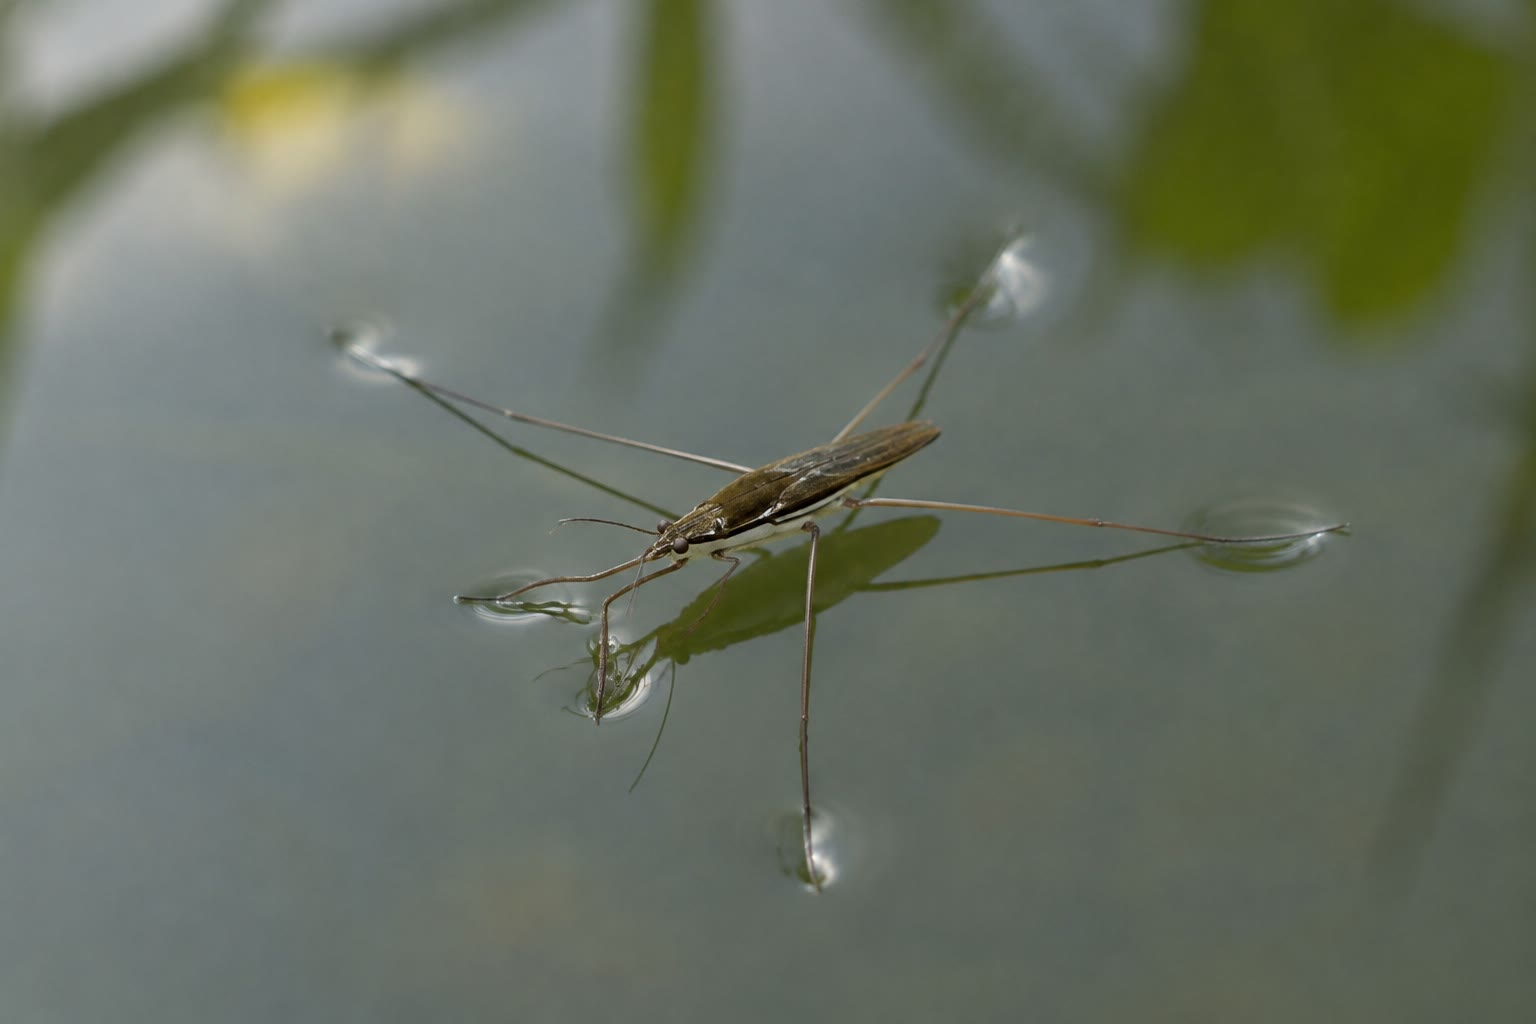
\includegraphics[width=0.6\linewidth]{images/book3/ai/b3-08-water-strider.jpg}

{\small किसी तालाब पर एक जलमापी कीट: उसके पैरों के नीचे के गड्ढे वही सतह
हैं जिसे हाइड्रोजन-बद्ध \omterm{def:b1:water-small-molecules:water}{जल} का संसंजन \omterm{def:b1:flowering-plant-organization:organs}{तना} हुआ रखता है।}
\end{omfigure}

\begin{example}[काम पर जलविरागी प्रभाव]\label{ex:b1:water-small-molecules:hydrophobic}
तेल को \omterm{def:b1:water-small-molecules:water}{जल} में हिलाइए और मिनटों में बूँदें आपस में मिल जाती हैं: \omterm{def:b1:water-small-molecules:water}{जल} उसे
निचोड़कर बाहर कर देता है जिससे वह बंध नहीं बना सकता। यही प्रभाव किसी
प्रोटीन को वलित करता है (उसके तैलीय अवशेष भीतर छिप जाते हैं,
\cref{ch:b1:proteins}), किसी झिल्ली को जोड़ता है (लिपिडों की पूँछें \omterm{def:b1:water-small-molecules:water}{जल} से
दूर इकट्ठी हो जाती हैं, \cref{ch:b1:lipids}), और दो मेल खाती आणविक सतहों
को साथ ले आता है। तेल को तेल की ओर कुछ खींचता नहीं; \omterm{def:b1:water-small-molecules:water}{जल} धकेलता है।
\end{example}

\section{दुर्बल बंध}

\begin{definition}[सहसंयोजी और असहसंयोजी बंध]\label{def:b1:water-small-molecules:bonds}
\emph{सहसंयोजी बंध}\index{सहसंयोजी बंध} दो परमाणुओं के बीच इलेक्ट्रॉनों
का एक युग्म साझा करता है और उसे तोड़ने में \qtyrange{300}{500}{kJ/mol}
लगते हैं: अणुओं के कंकाल सहसंयोजी होते हैं, और \omterm{def:b1:cell-unit-of-life:cell}{कोशिका} में उन्हें केवल
एंजाइम ही बनाते या तोड़ते हैं। \emph{असहसंयोजी बंध}\index{असहसंयोजी बंध}
वे दुर्बल, उत्क्रमणीय आकर्षण हैं जो अणुओं को \emph{एक-दूसरे से} थामते
हैं और उन्हें आकृति देते हैं: \emph{\omterm{def:b1:water-small-molecules:water}{हाइड्रोजन बंध}}
(\omterm{def:b1:water-small-molecules:water}{जल} में \qtyrange{4}{20}{kJ/mol}); विपरीत आवेशों के बीच का
\emph{आयनिक बंध}\index{आयनिक बंध} (\omterm{def:b1:water-small-molecules:water}{जल} में लगभग \qty{12}{kJ/mol}, जिसका
परावैद्युतांक आवेशों को अस्सी गुना परिरक्षित कर देता है); पास-पास आए
किन्हीं दो परमाणुओं के बीच के \emph{वान डर वाल्स}\index{वान डर वाल्स बल} आकर्षण
(हर एक \qtyrange{1}{4}{kJ/mol}, पर पूरी सतह पर जुड़ते हुए); और
\emph{\omterm{prop:b1:water-small-molecules:properties}{जलविरागी प्रभाव}}, जो बंध नहीं बल्कि \omterm{def:b1:water-small-molecules:water}{जल} द्वारा अध्रुवीय सतहों का
बहिष्करण है।
\end{definition}

\begin{proposition}[दुर्बल बंध ही जीवविज्ञान के बंध क्यों हैं]\label{prop:b1:water-small-molecules:weak}
\qty{37}{\celsius} पर ऊष्मीय ऊर्जा $RT = \qty{2.6}{kJ/mol}$ है। कोई
अकेला दुर्बल बंध इससे कुछ ही गुना है और माइक्रोसेकंडों में टूट जाता है;
पर दस बंध एक साथ, दो ऐसी सतहों पर जो एक-दूसरे में बैठती हों, घंटों थामे
रहते हैं। आणविक \emph{अभिज्ञान}\index{आणविक अभिज्ञान} --- किसी एंजाइम
का अपने क्रियाधार के लिए, किसी प्रतिरक्षी का अपने प्रतिजन के लिए, DNA की
एक लड़ी का अपनी पूरक के लिए --- पूरक सतहों के बीच एक साथ बने अनेक दुर्बल
बंधों पर टिका है, और इसीलिए वह एक ही साथ विशिष्ट है (सारे बंध केवल कोई
बैठती हुई सतह ही बनाती है) और उत्क्रमणीय भी (ऊष्मा, या कोई स्पर्धी, उसे
खोल देता है)। सौ गुना अधिक मज़बूत \omterm{def:b1:water-small-molecules:bonds}{सहसंयोजी बंध} स्थायी होते।
\end{proposition}

\begin{example}[किसी द्विकुंडली को पिघलाना]\label{ex:b1:water-small-molecules:melting}
DNA की दोनों लड़ियाँ प्रति \omterm{def:b1:water-small-molecules:ph}{क्षारक} युग्म दो या तीन \omterm{def:b1:water-small-molecules:water}{हाइड्रोजन बंधों} और
पड़ोसी युग्मों के स्तरण (\omterm{def:b1:water-small-molecules:bonds}{वान डर वाल्स}) से थमी हैं; कोई अकेला युग्म तुरंत
अलग हो जाता, पर एक पंक्ति में एक हज़ार युग्म तब तक थामे रहते हैं जब तक
ताप लगभग \qty{90}{\celsius} तक न पहुँच जाए, और ताप घटने पर वे ठीक उसी
पंजीकरण में फिर मिल जाते हैं (\cref{ch:b1:nucleic-acids})। विशिष्ट,
संख्या में मज़बूत, उत्क्रमणीय।
\end{example}

\section{अम्ल, क्षारक और बफ़र}

\begin{definition}[pH, अम्ल, क्षारक, p$K_a$]\label{def:b1:water-small-molecules:ph}
\omterm{def:b1:water-small-molecules:water}{जल} थोड़ा वियोजित होता है, $\mathrm{H_2O} \rightleftharpoons
\mathrm{H^+} + \mathrm{OH^-}$, और \qty{25}{\celsius} पर
$[\mathrm{H^+}][\mathrm{OH^-}] =
K_w = \qty{e-14}{mol^2/L^2}$ होता है।
\emph{pH}\index{pH} $-\log_{10}[\mathrm{H^+}]$ है: शुद्ध \omterm{def:b1:water-small-molecules:water}{जल} के लिए 7,
अम्लों के लिए कम, क्षारकों के लिए अधिक। कोई \emph{अम्ल}\index{अम्ल} $\mathrm{HA}$
एक प्रोटॉन छोड़ता है, $\mathrm{HA} \rightleftharpoons \mathrm{H^+} +
\mathrm{A^-}$, जिसका वियोजन स्थिरांक $K_a =
[\mathrm{H^+}][\mathrm{A^-}]/[\mathrm{HA}]$ है और
\emph{p$K_a$}\index{pKa@p$K_a$} $= -\log_{10}K_a$; और उसका संयुग्मी
\emph{क्षारक}\index{क्षारक} $\mathrm{A^-}$ एक प्रोटॉन लेता है। कोई प्रबल
अम्ल (HCl) पूरा वियोजित होता है; \omterm{def:b1:cell-unit-of-life:cell}{कोशिका} के अम्ल (कार्बोक्सिलिक अम्ल,
फ़ॉस्फ़ेट, अमोनियम) दुर्बल हैं, जिनका p$K_a$ 2 और 10 के बीच है।
\end{definition}

\begin{theorem}[हेंडरसन--हासेलबाख़]\label{thm:b1:water-small-molecules:hh}
\index{हेंडरसन--हासेलबाख़ समीकरण}
विलयन में किसी दुर्बल अम्ल के लिए,
\[
\mathrm{pH} = \mathrm{p}K_a + \log_{10}\frac{[\mathrm{A^-}]}{[\mathrm{HA}]} .
\]
$\mathrm{pH} = \mathrm{p}K_a$ पर अम्ल आधा वियोजित होता है; उससे एक \omterm{def:b1:water-small-molecules:ph}{pH}
मात्रक ऊपर \qty{91}{\%} वियोजित, और एक नीचे \qty{9}{\%}।
\end{theorem}
\begin{proof}
$K_a = [\mathrm{H^+}][\mathrm{A^-}]/[\mathrm{HA}]$ का लघुगणक लीजिए:
$\log K_a = \log[\mathrm{H^+}] + \log([\mathrm{A^-}]/[\mathrm{HA}])$,
यानी $-\mathrm{p}K_a = -\mathrm{pH} + \log([\mathrm{A^-}]/[\mathrm{HA}])$।
यह अनुपात $1$, $10$ और $0.1$ होता है, क्रमशः \omterm{def:b1:water-small-molecules:ph}{pH} $= \mathrm{p}K_a$,
$\mathrm{p}K_a + 1$ और $\mathrm{p}K_a - 1$ पर।
\end{proof}

\begin{definition}[बफ़र]\label{def:b1:water-small-molecules:buffer}
\emph{बफ़र}\index{बफ़र} वह विलयन है जिसमें कोई दुर्बल अम्ल और उसका
संयुग्मी \omterm{def:b1:water-small-molecules:ph}{क्षारक} तुलनीय मात्राओं में हों; वह \omterm{def:b1:water-small-molecules:ph}{pH} के परिवर्तन का प्रतिरोध
करता है, क्योंकि मिलाया गया $\mathrm{H^+}$ $\mathrm{A^-}$ ले लेता है और
मिलाया गया $\mathrm{OH^-}$ $\mathrm{HA}$। वह p$K_a$ के एक मात्रक के भीतर
सबसे अच्छा काम करता है, और उसकी \emph{क्षमता} उस युग्म की कुल सांद्रता के
साथ बढ़ती है। \omterm{def:b1:cell-unit-of-life:cell}{कोशिका} के बफ़र: फ़ॉस्फ़ेट
($\mathrm{H_2PO_4^-}/\mathrm{HPO_4^{2-}}$, p$K_a$ 6.8) और \omterm{def:b1:cell-unit-of-life:cell}{कोशिकाओं} के
भीतर प्रोटीनों की पार्श्व शृंखलाएँ; तथा रक्त में बाइकार्बोनेट
($\mathrm{CO_2}/\mathrm{HCO_3^-}$, प्रभावी p$K_a$ 6.1), जिसका अम्ल
साथी एक गैस है जिसे फेफड़े हटा सकते हैं।
\end{definition}

\begin{omfigure}
\begin{tikzpicture}
\begin{axis}[
  width=0.86\linewidth, height=6.2cm,
  axis x line=bottom, axis y line=left,
  xmin=0, xmax=1, ymin=3, ymax=11,
  xlabel={उदासीन किए गए अम्ल का भिन्न (मिलाए गए $\mathrm{OH^-}$ के तुल्यांक)}, ylabel={pH},
  xlabel style={font=\small, at={(axis description cs:0.5,-0.12)}, anchor=north},
  ylabel style={font=\small},
  tick label style={font=\small}, xtick={0,0.25,0.5,0.75,1}, ytick={3,4,5,6,7,8,9,10,11},
  clip=false,
]
\addplot[very thick, omDef, domain=0.02:0.98, samples=120] {6.8 + log10(x/(1-x))};
\draw[dashed, gray] (axis cs:0,6.8) -- (axis cs:0.5,6.8);
\draw[dashed, gray] (axis cs:0.5,3) -- (axis cs:0.5,6.8);
\node[font=\scriptsize, anchor=south west] at (axis cs:0.02,6.85) {अर्ध-उदासीनीकरण पर pH $=$ p$K_a$ $= 6.8$};
\draw[<->, thick, omThm] (axis cs:0.09,5.8) -- (axis cs:0.91,7.8);
\node[font=\scriptsize, omThm, anchor=north west, align=left] at (axis cs:0.55,5.7) {बफ़र-परास:\\ p$K_a \pm 1$, चपटा वक्र};
\end{axis}
\end{tikzpicture}

{\small किसी \omterm{def:b1:water-small-molecules:ph}{क्षारक} द्वारा किसी दुर्बल अम्ल (फ़ॉस्फ़ेट, p$K_a$ 6.8) का
अनुमापन। वक्र p$K_a$ के आसपास चपटा है: वहाँ \omterm{def:b1:water-small-molecules:ph}{क्षारक} मिलाने पर \omterm{def:b1:water-small-molecules:ph}{क्षारक} और
अम्ल का अनुपात बदलता है पर \omterm{def:b1:water-small-molecules:ph}{pH} मुश्किल से। परास के बाहर \omterm{def:b1:water-small-molecules:ph}{pH} स्वतंत्र रूप
से झूलता है।}
\end{omfigure}

\begin{omfigure}
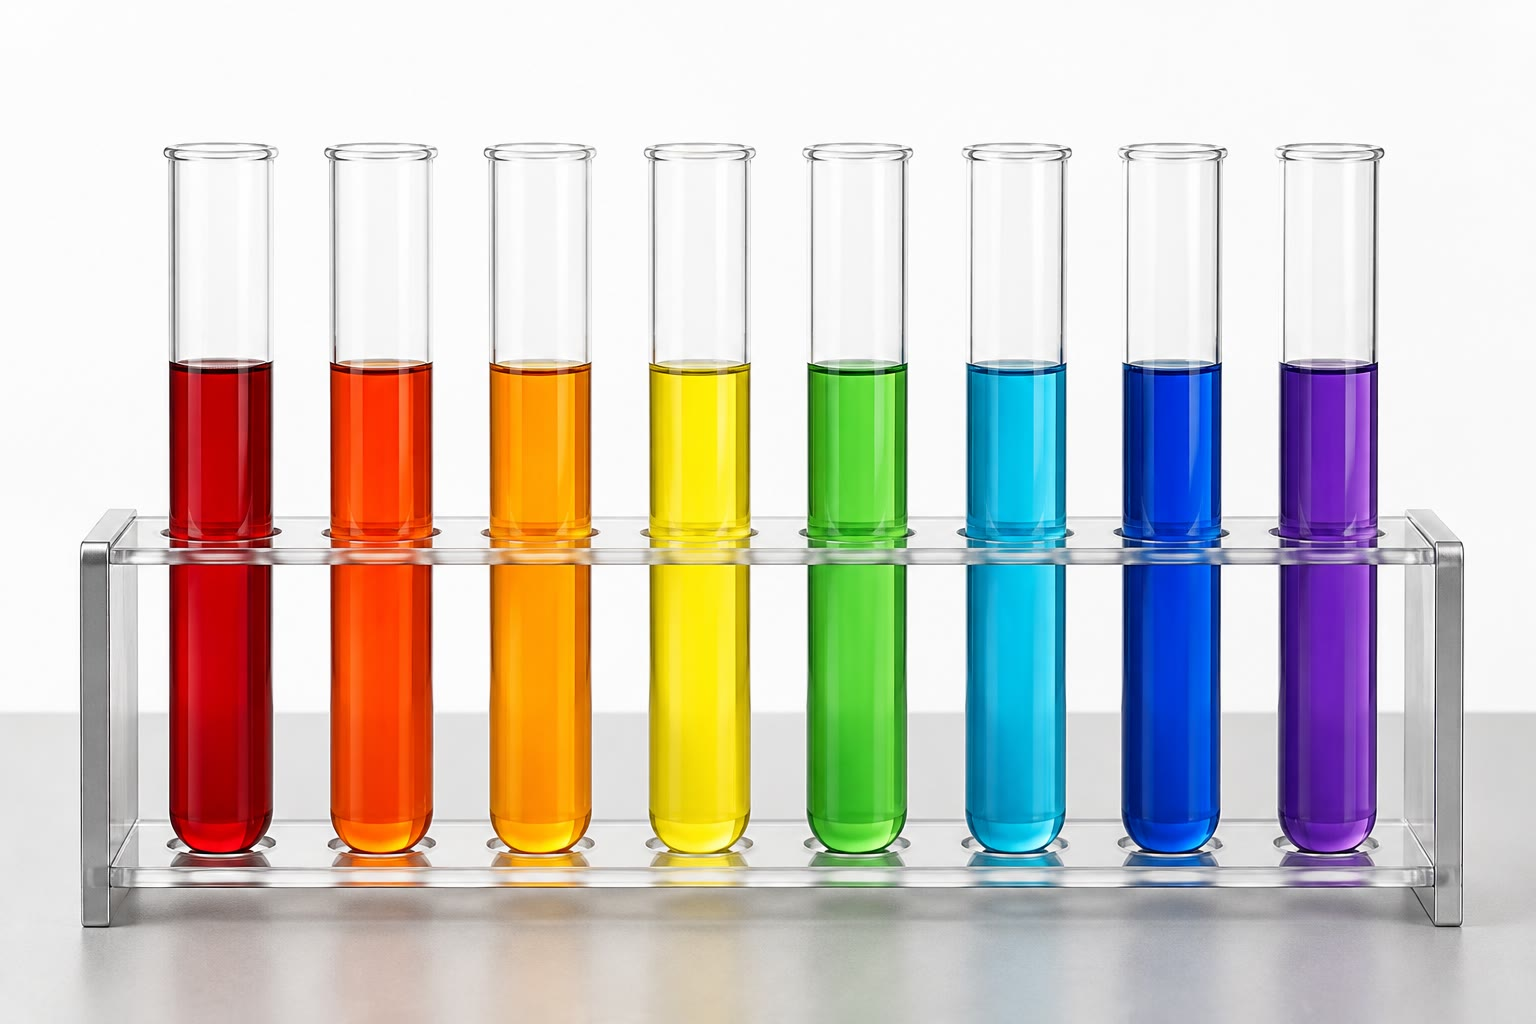
\includegraphics[width=0.6\linewidth]{images/book3/ai/b3-08-indicator-tubes.jpg}

{\small सार्वत्रिक सूचक से दिखाई गई \omterm{def:b1:water-small-molecules:ph}{pH} मापनी: \omterm{def:b1:water-small-molecules:ph}{pH} 2 पर लाल से \omterm{def:b1:water-small-molecules:ph}{pH} 12 पर
बैंगनी तक। जठर रस 1--2 पर है, मूत्र 5--8, रक्त 7.4, छोटी आँत 8,
\omterm{def:b1:eukaryotic-cell:organelle}{कोशिकाद्रव} 7.2, \omterm{def:b1:eukaryotic-cell:endomembrane}{लयनकाय} 5, प्रकाश में थाइलेकॉइड की अवकाशिका 5, और पीठिका
8।}
\end{omfigure}

\begin{method}[बफ़र का अंकगणित]\label{met:b1:water-small-molecules:bufferarith}
\begin{enumerate}
  \item अम्ल--क्षारक युग्म और कार्यरत ताप पर उसका p$K_a$ पहचानिए।
  \item \omterm{def:b1:water-small-molecules:ph}{pH} से \omterm{def:b1:water-small-molecules:ph}{क्षारक}/अम्ल का अनुपात पाने के लिए, या सांद्रताओं से \omterm{def:b1:water-small-molecules:ph}{pH}
        पाने के लिए, हेंडरसन--हासेलबाख़ लगाइए।
  \item कोई प्रबल अम्ल मिलाने के लिए: उसकी मात्रा \omterm{def:b1:water-small-molecules:ph}{क्षारक} में से घटाइए
        और अम्ल में जोड़िए, फिर \omterm{def:b1:water-small-molecules:ph}{pH} फिर से निकालिए। कोई प्रबल \omterm{def:b1:water-small-molecules:ph}{क्षारक}
        मिलाने के लिए: उल्टा।
  \item यदि कोई एक साथी तंत्र से निकल सकता हो (साँस से बाहर जाती कार्बन
        डाइऑक्साइड, उत्सर्जित अमोनिया), तो तंत्र \emph{विवृत} है: उस
        साथी को जमा होने देने के बजाय उसके थोपे गए मान पर रखिए। विवृत
        \omterm{def:b1:water-small-molecules:buffer}{बफ़र} \omterm{def:b1:water-small-molecules:ph}{pH} को बंद \omterm{def:b1:water-small-molecules:buffer}{बफ़रों} से कहीं बेहतर थामते हैं।
\end{enumerate}
\end{method}

\begin{example}[रक्त]\label{ex:b1:water-small-molecules:blood}
धमनी रक्त में \qty{24}{mmol/L} बाइकार्बोनेट है और \qty{1.2}{mmol/L} पर
घुली $\mathrm{CO_2}$ (जिसे फेफड़े तय करते हैं): $\mathrm{pH} =
6.1 + \log(24/1.2) = 6.1 + 1.30 = 7.4$। \qty{5}{mmol/L} अम्ल मिलाने पर
\qty{5}{mmol/L} बाइकार्बोनेट $\mathrm{CO_2}$ में बदल जाता है; यदि फेफड़े
उस $\mathrm{CO_2}$ को उड़ा दें और घुला मान थामे रखें तो \omterm{def:b1:water-small-molecules:ph}{pH}
$6.1 + \log(19/1.2) = 7.30$ हो जाता है; और किसी बंद फ़्लास्क में
$\mathrm{CO_2}$ बढ़कर \qty{6.2}{mmol/L} हो जाती और \omterm{def:b1:water-small-molecules:ph}{pH} गिरकर
$6.1 + \log(19/6.2) =
6.59$। फ़र्क़ फेफड़े डालते हैं।
\end{example}

\section{छोटे जैव-अणु}

\begin{definition}[क्रियात्मक समूह]\label{def:b1:water-small-molecules:groups}
\omterm{def:b1:cell-unit-of-life:cell}{कोशिका} के कार्बनिक अणु कार्बन के कंकाल हैं जो \emph{क्रियात्मक
समूहों}\index{क्रियात्मक समूह} का एक छोटा समुच्चय धारण करते हैं और जो
उनका रसायन तय करते हैं:
\begin{center}
\small
\begin{tabular}{llll}
\hline
समूह & सूत्र & गुण & कहाँ मिलता है \\
\hline
हाइड्रॉक्सिल & $-\mathrm{OH}$ & \omterm{def:b1:water-small-molecules:water}{ध्रुवीय}, H-बंधकारी & शर्कराएँ, ऐल्कोहॉल \\
कार्बोनिल & $>\!\mathrm{C{=}O}$ & \omterm{def:b1:water-small-molecules:water}{ध्रुवीय}, क्रियाशील & ऐल्डोस, कीटोस \\
कार्बोक्सिल & $-\mathrm{COOH}$ & अम्ल (p$K_a \approx 4$) & वसा अम्ल, ऐमीनो अम्ल \\
ऐमीनो & $-\mathrm{NH_2}$ & \omterm{def:b1:water-small-molecules:ph}{क्षारक} (p$K_a \approx 9$) & ऐमीनो अम्ल \\
फ़ॉस्फ़ेट & $-\mathrm{OPO_3^{2-}}$ & आवेशित, ऊर्जा-समृद्ध जोड़ & न्यूक्लियोटाइड, \omterm{def:b1:water-small-molecules:atp}{ATP} \\
सल्फ़हाइड्रिल & $-\mathrm{SH}$ & S--S सेतु बनाता है & सिस्टीन \\
मेथिल & $-\mathrm{CH_3}$ & अध्रुवीय & लिपिड, DNA के चिह्न \\
\hline
\end{tabular}
\end{center}
\omterm{def:b1:cell-unit-of-life:cell}{कोशिका} के \omterm{def:b1:water-small-molecules:ph}{pH} पर कार्बोक्सिल समूह आयनित रहते हैं ($-\mathrm{COO^-}$) और
ऐमीनो समूह प्रोटॉनित ($-\mathrm{NH_3^+}$)।
\end{definition}

\begin{proposition}[निर्माण-खंडों के चार कुल]\label{prop:b1:water-small-molecules:families}
किसी \omterm{def:b1:cell-unit-of-life:cell}{कोशिका} का लगभग सारा कार्बनिक पदार्थ चार प्रकार के छोटे अणुओं से बना
है, जिनमें से हर एक कुछ सौ डाल्टन का है: \emph{शर्कराएँ}
(\cref{ch:b1:carbohydrates}), \emph{वसा अम्ल} (\cref{ch:b1:lipids}),
\emph{ऐमीनो अम्ल} (\cref{ch:b1:proteins}) और \emph{न्यूक्लियोटाइड}
(\cref{ch:b1:nucleic-acids})। इनमें से तीन \emph{बहुलकों} में जुड़ते
हैं --- बहुशर्कराएँ, प्रोटीन, न्यूक्लिक अम्ल --- और वह जोड़
\emph{संघनन}\index{संघनन} से बनता है (यानी एक जल-अणु के ह्रास के साथ
बना बंध), जबकि \emph{जल-अपघटन}\index{जल-अपघटन} उन्हें अलग करता है
(यानी \omterm{def:b1:water-small-molecules:water}{जल} जोड़कर तोड़ा गया बंध)। संघनन चढ़ाई है और \omterm{def:b1:water-small-molecules:atp}{ATP} से चुकाया जाता है; \omterm{prop:b1:water-small-molecules:families}{जल-अपघटन} ढलान है
और उसे केवल एक एंजाइम चाहिए।
\end{proposition}

\begin{omfigure}
\begin{tikzpicture}[font=\small, >=Stealth, line cap=round,
  mono/.style={draw, thick, rounded corners=3pt, minimum width=16mm, minimum height=8mm, fill=omDef!12}]
  \node[mono] (a) at (0,0) {एकलक};
  \node[mono] (b) at (2.4,0) {एकलक};
  \node[font=\footnotesize] at (1.2,0.55) {$-\mathrm{OH}$ \quad $\mathrm{H}-$};
  \draw[->, very thick, omExo] (3.6,0.15) -- (5.6,0.15) node[midway, above, font=\footnotesize, align=center] {संघनन\\ (ATP चुकाया)};
  \draw[->, very thick, omThm] (5.6,-0.15) -- (3.6,-0.15) node[midway, below, font=\footnotesize, align=center] {जल-अपघटन\\ (केवल एंजाइम)};
  \node[mono, minimum width=34mm] (ab) at (7.6,0) {एकलक---एकलक};
  \node[font=\footnotesize] at (7.6,0.55) {सहसंयोजी जोड़};
  \node[font=\footnotesize, omDef] at (9.9,-0.6) {$+\ \mathrm{H_2O}$};
\end{tikzpicture}

{\small संघनन दो निर्माण-खंडों को एक जल-अणु के ह्रास के साथ जोड़ता है;
\omterm{prop:b1:water-small-molecules:families}{जल-अपघटन} एक जल-अणु जोड़कर उन्हें अलग करता है। शर्कराएँ, ऐमीनो अम्ल और
न्यूक्लियोटाइड इसी तरह बहुलकित होते हैं।}
\end{omfigure}

\begin{example}[कोशिका की सूची]\label{ex:b1:water-small-molecules:inventory}
किसी जीवाणु के शुष्क द्रव्यमान में प्रोटीन \qty{55}{\%} हैं, RNA
\qty{20}{\%}, DNA \qty{3}{\%}, लिपिड \qty{9}{\%}, बहुशर्कराएँ
\qty{5}{\%}, और बाक़ी छोटे अणु तथा आयन। अणुओं की संख्या के हिसाब से चित्र
उल्टा हो जाता है: नैनोमोलर से लेकर एक मोल प्रति लीटर के दसवें भाग तक की
सांद्रताओं पर एक हज़ार प्रकार के छोटे उपापचयज और आयन उन अधिकांश अणुओं को
बनाते हैं जो \omterm{def:b1:water-small-molecules:water}{जल} नहीं हैं। पोटैशियम \qty{150}{mmol/L} पर है, ग्लूटामेट
\qty{100}{mmol/L}, \omterm{def:b1:water-small-molecules:atp}{ATP} \qty{5}{mmol/L}, और कोई अनुलेखन कारक प्रति
\omterm{def:b1:cell-unit-of-life:cell}{कोशिका} कुछ ही अणुओं पर।
\end{example}

\section{ऊर्जा: मुक्त ऊर्जा और ATP}

\begin{proposition}[किसी अभिक्रिया की मुक्त ऊर्जा]\label{prop:b1:water-small-molecules:gibbs}
\index{मुक्त ऊर्जा}
अचर ताप और दाब पर कोई अभिक्रिया स्वतःस्फूर्त रूप से उस दिशा में चलती है
जो गिब्स \omterm{prop:b1:water-small-molecules:gibbs}{मुक्त ऊर्जा} $G$ को घटाती है।
$\mathrm{A} + \mathrm{B} \rightleftharpoons \mathrm{C} + \mathrm{D}$ के लिए,
\[
\Delta G = \Delta G^{\circ\prime} + RT\ln\frac{[\mathrm{C}][\mathrm{D}]}{[\mathrm{A}][\mathrm{B}]},
\]
जिसमें $\Delta G^{\circ\prime}$ मानक मुक्त-ऊर्जा परिवर्तन है
(सारी सांद्रताएँ \qty{1}{mol/L}, \omterm{def:b1:water-small-molecules:ph}{pH} 7) और लघुगणकीय पद असली सांद्रताओं के
लिए संशोधन करता है। साम्य पर $\Delta G = 0$ होता है, इसलिए
$\Delta G^{\circ\prime} = -RT\ln K'_{\text{सा}}$: और
$\Delta G^{\circ\prime}$ के हर \qty{5.7}{kJ/mol} पर साम्य स्थिरांक दस
गुना खिसक जाता है। $\Delta G$ बताता है कि कोई अभिक्रिया किस ओर जा सकती
है, कितनी तेज़ नहीं: वह एंजाइम का काम है (\cref{ch:b1:enzymes})।
\end{proposition}
\begin{proof}
हर स्पीशीज़ का रासायनिक विभव $\mu = \mu^\circ + RT\ln c$ है
(भौतिकी पाठ्यक्रम का आदर्श-विलयन परिणाम); $\Delta G$ उत्पादों के विभवों
के योग में से अभिकारकों के विभवों का योग घटाने पर मिलता है, जिससे सूत्र
निकल आता है; और साम्य पर उसे शून्य रखने पर $K'_{\text{सा}}$ से संबंध मिल
जाता है।
\end{proof}

\begin{definition}[ATP, युग्मन]\label{def:b1:water-small-molecules:atp}
\emph{ATP}\index{ATP} (एडेनोसिन ट्राइफ़ॉस्फ़ेट) एक न्यूक्लियोटाइड है
(\cref{ch:b1:nucleic-acids}) जो एक पंक्ति में तीन फ़ॉस्फ़ेट धारण करता
है; बाहर के दोनों बंध \emph{फ़ॉस्फ़ोऐनहाइड्राइड}\index{फ़ॉस्फ़ोऐनहाइड्राइड बंध}
बंध हैं जिनके \omterm{prop:b1:water-small-molecules:families}{जल-अपघटन}, $\mathrm{ATP} + \mathrm{H_2O} \to \mathrm{ADP} +
\mathrm{P_i}$, का $\Delta G^{\circ\prime} = \qty{-30.5}{kJ/mol}$ है और
किसी \omterm{def:b1:cell-unit-of-life:cell}{कोशिका} की सांद्रताओं पर $\Delta G \approx \qty{-50}{kJ/mol}$।
ATP \omterm{def:b1:cell-unit-of-life:cell}{कोशिका} की \emph{ऊर्जा मुद्रा}\index{ऊर्जा मुद्रा} है:
अपचय उसे बनाता है (\cref{ch:b1:respiration-fermentation}), और
जैवसंश्लेषण, अभिगमन तथा गति उसे ख़र्च करते हैं। किसी चढ़ाई वाली
अभिक्रिया को चलाया जाता है, उसे किसी साझा मध्यवर्ती के माध्यम से ATP के
\omterm{prop:b1:water-small-molecules:families}{जल-अपघटन} से \emph{युग्मित}\index{ऊर्जा युग्मन} करके, ताकि दोनों के
$\Delta G$ का योग ऋणात्मक हो।
\end{definition}

\begin{example}[ATP का जल-अपघटन इतना कुछ क्यों छोड़ता है]\label{ex:b1:water-small-molecules:whyatp}
तीन कारण: \omterm{def:b1:water-small-molecules:atp}{ATP} के फ़ॉस्फ़ेटों के चारों ऋण आवेश एक-दूसरे को प्रतिकर्षित
करते हैं और कटने से उन्हें राहत मिल जाती है; उत्पाद $\mathrm{ADP}$ और
$\mathrm{P_i}$ अनुनाद तथा जलयोजन से ऐनहाइड्राइड की तुलना में बेहतर
स्थायी होते हैं; और \omterm{def:b1:cell-unit-of-life:cell}{कोशिका} \omterm{def:b1:water-small-molecules:atp}{ATP} को ADP तथा फ़ॉस्फ़ेट के साथ उसके साम्य से
एक हज़ार गुना ऊपर रखती है। अंतिम पद सबसे बड़ा है: \omterm{def:b1:water-small-molecules:atp}{ATP} \qty{5}{mmol/L}
पर, ADP \qty{1}{mmol/L} पर, $\mathrm{P_i}$
\qty{10}{mmol/L} पर,
$\Delta G = -30.5 + 2.58\ln\frac{10^{-3}\times 10^{-2}}{5\times 10^{-3}}
= -30.5 - 16 = \qty{-46.5}{kJ/mol}$।
\end{example}

\begin{example}[युग्मन]\label{ex:b1:water-small-molecules:coupling}
ग्लूकोज़ $+\ \mathrm{P_i} \to$ ग्लूकोज़-6-फ़ॉस्फ़ेट $+\ \mathrm{H_2O}$
का $\Delta G^{\circ\prime} = \qty{+13.8}{kJ/mol}$ है: साम्य पर लगभग
कोई ग्लूकोज़ फ़ॉस्फ़ोरिलित नहीं होता। इसके बजाय हेक्सोकाइनेज़
फ़ॉस्फ़ेट सीधे \omterm{def:b1:water-small-molecules:atp}{ATP} से हस्तांतरित करता है: ग्लूकोज़ $+$ \omterm{def:b1:water-small-molecules:atp}{ATP} $\to$
ग्लूकोज़-6-फ़ॉस्फ़ेट $+$ ADP, $\Delta G^{\circ\prime} = 13.8 - 30.5 =
\qty{-16.7}{kJ/mol}$, साम्य स्थिरांक $800$, और अभिक्रिया लगभग पूरी।
फ़ॉस्फ़ेट कभी मुक्त नहीं दिखता: दोनों अभिक्रियाएँ एक ही हैं।
\end{example}

\section{अभ्यास}

\begin{exercise}[$\star$]\label{exo:b1:water-small-molecules:1}
जल-अणु की संरचना से समझाइए कि \omterm{def:b1:water-small-molecules:water}{जल} लवणों के लिए अच्छा विलायक और तेलों के
लिए घटिया विलायक क्यों है।
\end{exercise}

\begin{exercise}[$\star$]\label{exo:b1:water-small-molecules:2}
असहसंयोजी अंतःक्रियाओं के चारों प्रकारों को सामर्थ्य के क्रम में रखिए और
हर एक की एक जैविक भूमिका बताइए।
\end{exercise}

\begin{exercise}[$\star$]\label{exo:b1:water-small-molecules:3}
उस विलयन का \omterm{def:b1:water-small-molecules:ph}{pH} निकालिए जिसमें $[\mathrm{H^+}] = \qty{4e-8}{mol/L}$ है,
और \omterm{def:b1:water-small-molecules:ph}{pH} 1.5 के जठर रस में $[\mathrm{H^+}]$ भी।
\end{exercise}

\begin{exercise}[$\star$]\label{exo:b1:water-small-molecules:4}
अनुमापन वाले आलेख से बताइए कि फ़ॉस्फ़ेट \omterm{def:b1:water-small-molecules:buffer}{बफ़र} \omterm{def:b1:water-small-molecules:ph}{pH} के किस परास में काम करता
है, और \omterm{def:b1:water-small-molecules:ph}{pH} 7.4 पर \omterm{def:b1:water-small-molecules:ph}{क्षारक} तथा अम्ल का अनुपात क्या है।
\end{exercise}

\begin{exercise}[$\star\star$]\label{exo:b1:water-small-molecules:5}
ऐसीटिक अम्ल का p$K_a$ 4.76 है। \omterm{def:b1:water-small-molecules:ph}{pH} 4.76 पर, \omterm{def:b1:water-small-molecules:ph}{pH} 7.2 (\omterm{def:b1:eukaryotic-cell:organelle}{कोशिकाद्रव}) पर और
\omterm{def:b1:water-small-molecules:ph}{pH} 2 (आमाशय) पर उसका कितना भिन्न आयनित है? कौन-सा रूप झिल्ली अधिक आसानी
से पार करता है, और ऐसीटिक अम्ल कहाँ अवशोषित होगा?
\end{exercise}

\begin{exercise}[$\star\star$]\label{exo:b1:water-small-molecules:6}
किसी \omterm{def:b1:water-small-molecules:buffer}{बफ़र} में \qty{50}{mmol/L} $\mathrm{HPO_4^{2-}}$ और
\qty{50}{mmol/L} $\mathrm{H_2PO_4^-}$ है (p$K_a$ 6.8)। उसका \omterm{def:b1:water-small-molecules:ph}{pH}
निकालिए। \qty{10}{mmol/L} HCl मिलाने के बाद का \omterm{def:b1:water-small-molecules:ph}{pH} निकालिए, और वही HCl
शुद्ध \omterm{def:b1:water-small-molecules:water}{जल} में मिलाने के बाद का भी।
\end{exercise}

\begin{exercise}[$\star\star$]\label{exo:b1:water-small-molecules:7}
पसीने का वाष्पन किसी धावक को ठंडा करता है। \qty{500}{kJ} हटाने के लिए
कितना पसीना वाष्पित होना चाहिए? \omterm{def:b1:water-small-molecules:water}{हाइड्रोजन बंधों} से समझाइए कि \omterm{def:b1:water-small-molecules:water}{जल} की
वाष्पन ऊष्मा इतनी बड़ी क्यों है।
\end{exercise}

\begin{exercise}[$\star\star$]\label{exo:b1:water-small-molecules:8}
अभिक्रिया ग्लूकोज़-1-फ़ॉस्फ़ेट $\to$ ग्लूकोज़-6-फ़ॉस्फ़ेट का
\qty{25}{\celsius} पर $K'_{\text{सा}} = 19$ है।
$\Delta G^{\circ\prime}$ निकालिए। जिस \omterm{def:b1:cell-unit-of-life:cell}{कोशिका} में
ग्लूकोज़-6-फ़ॉस्फ़ेट \qty{2}{mmol/L} पर और ग्लूकोज़-1-फ़ॉस्फ़ेट
\qty{0.02}{mmol/L} पर हो, उसमें $\Delta G$ निकालिए और बताइए कि
अभिक्रिया किस ओर चलती है।
\end{exercise}

\begin{exercise}[$\star\star$]\label{exo:b1:water-small-molecules:9}
कोई झील ऊपर से नीचे की ओर क्यों जमती है, और यह उसकी मछलियों के लिए
क्यों मायने रखता है? जिस संसार में बर्फ़ डूबती, वहाँ क्या होता?
\end{exercise}

\begin{exercise}[$\star\star\star$]\label{exo:b1:water-small-molecules:10}
उस पेशी \omterm{def:b1:cell-unit-of-life:cell}{कोशिका} में \omterm{def:b1:water-small-molecules:atp}{ATP} के \omterm{prop:b1:water-small-molecules:families}{जल-अपघटन} का $\Delta G$ निकालिए जिसमें
\qty{37}{\celsius} पर \omterm{def:b1:water-small-molecules:atp}{ATP} \qty{8}{mmol/L}, ADP \qty{0.9}{mmol/L} और
$\mathrm{P_i}$ \qty{8}{mmol/L} है; फिर उस थकी पेशी में जिसमें
\omterm{def:b1:water-small-molecules:atp}{ATP} \qty{5}{mmol/L}, ADP \qty{3}{mmol/L} और $\mathrm{P_i}$
\qty{30}{mmol/L} है। थकान ने प्रति \omterm{def:b1:water-small-molecules:atp}{ATP} उपलब्ध ऊर्जा का क्या किया है?
\end{exercise}

\begin{exercise}[$\star\star\star$]\label{exo:b1:water-small-molecules:11}
\omterm{def:b1:water-small-molecules:ph}{pH} 7.2 और \qty{37}{\celsius} की किसी \omterm{def:b1:cell-unit-of-life:cell}{कोशिका} का भीतरी आयतन
\qty{1000}{\micro m^3} है। उसमें कितने मुक्त $\mathrm{H^+}$ आयन हैं?
इसकी तुलना उसके $\num{3e9}$ बफ़रकारी समूहों से कीजिए। इस तुलना से
``किसी \omterm{def:b1:cell-unit-of-life:cell}{कोशिका} का \omterm{def:b1:water-small-molecules:ph}{pH}'' के अर्थ के बारे में क्या पता चलता है?
\end{exercise}

\begin{exercise}[$\star\star\star$]\label{exo:b1:water-small-molecules:12}
``जीवन अभिक्रियाओं को साम्य से दूर रखने का एक ढंग है।'' \omterm{def:b1:water-small-molecules:atp}{ATP} के
सांद्रता-अनुपात, युग्मन, और उस \omterm{def:b1:cell-unit-of-life:cell}{कोशिका} का क्या होता है जिसका \omterm{def:b1:water-small-molecules:atp}{ATP} ADP के
साथ साम्य पर पहुँच जाए --- इनकी सहायता से एक अनुच्छेद में चर्चा कीजिए।
\end{exercise}

\section{समस्या: बफ़र के रूप में रक्त}

\begin{problem}[{सप्ताहांत समस्या --- किसी दौड़ के दौरान pH 7.40 पर
पाँच लीटर रक्त: बाइकार्बोनेट, कार्बन डाइऑक्साइड, फेफड़े और गुर्दे, और
अंत में किसी दिए गए लैक्टेट भार पर pH का खिसकाव}]
\label{pb:b1:water-small-molecules:1}
धमनी रक्त: \omterm{def:b1:water-small-molecules:ph}{pH} 7.40, बाइकार्बोनेट $[\mathrm{HCO_3^-}] =
\qty{24}{mmol/L}$, घुली कार्बन डाइऑक्साइड $[\mathrm{CO_2}] =
\qty{1.2}{mmol/L}$ (जो उसके आंशिक दाब के समानुपाती है: \qty{40}{mmHg}
का आंशिक दाब \qty{1.2}{mmol/L} देता है)। बाइकार्बोनेट तंत्र का प्रभावी
p$K_a$ 6.1 है: $\mathrm{CO_2} + \mathrm{H_2O}
\rightleftharpoons \mathrm{H^+} + \mathrm{HCO_3^-}$। रक्त का आयतन
\qty{5}{L}। प्लाज़्मा प्रोटीन और हीमोग्लोबिन एक दूसरा \omterm{def:b1:water-small-molecules:buffer}{बफ़र} जोड़ते हैं
जिसकी क्षमता प्रति लीटर प्रति \omterm{def:b1:water-small-molecules:ph}{pH} मात्रक \qty{25}{mmol} $\mathrm{H^+}$
है। कोई दौड़ मिनट भर में \qty{60}{mmol} लैक्टिक अम्ल (जो रक्त के \omterm{def:b1:water-small-molecules:ph}{pH} पर
प्रबल अम्ल है) रक्त में छोड़ देती है।

\medskip
\noindent\textbf{भाग I --- विश्राम की अवस्था।}
\begin{enumerate}
  \item बाइकार्बोनेट और कार्बन डाइऑक्साइड के मानों से धमनी रक्त का \omterm{def:b1:water-small-molecules:ph}{pH}
        जाँचिए।
  \item \omterm{def:b1:water-small-molecules:ph}{pH} 7.40 पर $[\mathrm{H^+}]$ नैनोमोल प्रति लीटर में निकालिए।
  \item पूरे रक्त-आयतन में कितने मुक्त प्रोटॉन हैं? इसकी तुलना
        \qty{120}{mmol} बाइकार्बोनेट से कीजिए।
  \item बाइकार्बोनेट का घुली कार्बन डाइऑक्साइड से अनुपात निकालिए, और
        बफ़र-युग्म का वह भिन्न भी जो \omterm{def:b1:water-small-molecules:ph}{क्षारक} के रूप में मौजूद है।
  \item शिरा रक्त में $\mathrm{CO_2}$ का आंशिक दाब \qty{46}{mmHg} है
        और बाइकार्बोनेट \qty{25}{mmol/L}। उसका \omterm{def:b1:water-small-molecules:ph}{pH} निकालिए।
  \item 6.1 का p$K_a$, जो रक्त के \omterm{def:b1:water-small-molecules:ph}{pH} से एक मात्रक से अधिक नीचे है, इस
        \omterm{def:b1:water-small-molecules:buffer}{बफ़र} के लिए शरीर में बाधा क्यों नहीं है, जबकि किसी फ़्लास्क में
        होता?
\end{enumerate}

\medskip
\noindent\textbf{भाग II --- दौड़, बंद तंत्र।}
पहले मान लीजिए कि कोई कार्बन डाइऑक्साइड बाहर नहीं जा सकती: बाइकार्बोनेट
द्वारा लिया गया हर प्रोटॉन घुली $\mathrm{CO_2}$ बन जाता है।
\begin{enumerate}[resume]
  \item रक्त में जोड़ी गई लैक्टिक अम्ल की सांद्रता निकालिए।
  \item यदि सारा अम्ल बाइकार्बोनेट से \omterm{def:b1:water-small-molecules:buffer}{बफ़र} हो जाए तो नया बाइकार्बोनेट
        और नई घुली $\mathrm{CO_2}$ निकालिए।
  \item परिणामी \omterm{def:b1:water-small-molecules:ph}{pH} निकालिए।
  \item वही अम्ल \qty{5}{L} शुद्ध \omterm{def:b1:water-small-molecules:water}{जल} में जो \omterm{def:b1:water-small-molecules:ph}{pH} देता, वह निकालिए।
  \item क्या बंद बाइकार्बोनेट तंत्र इस भार के लिए अच्छा \omterm{def:b1:water-small-molecules:buffer}{बफ़र} है? \omterm{def:b1:water-small-molecules:ph}{pH} के
        खिसकाव से इसे मात्रात्मक रूप में बताइए।
  \item \omterm{def:b1:water-small-molecules:ph}{pH} 7.40 और प्रश्न 9 के \omterm{def:b1:water-small-molecules:ph}{pH} के बीच $[\mathrm{H^+}]$ का परिवर्तन
        निकालिए, और जोड़े गए प्रोटॉनों का वह भिन्न भी जो विलयन में
        मुक्त रह जाता है।
\end{enumerate}

\medskip
\noindent\textbf{भाग III --- दौड़, \omterm{def:b1:organism-environment:organism}{विवृत तंत्र}।}
अब फेफड़े अतिरिक्त को उड़ाकर घुली $\mathrm{CO_2}$ को \qty{1.2}{mmol/L}
पर थामे रखते हैं।
\begin{enumerate}[resume]
  \item बाइकार्बोनेट को उसके नए मान पर और $\mathrm{CO_2}$ को
        \qty{1.2}{mmol/L} पर थामकर \omterm{def:b1:water-small-molecules:ph}{pH} निकालिए।
  \item उस मान को थामने के लिए फेफड़ों को, विश्राम के निर्गम से ऊपर,
        कितने मिलीमोल $\mathrm{CO_2}$ हटाने होंगे?
  \item विश्राम का निर्गम प्रति मिनट \qty{10}{mmol} $\mathrm{CO_2}$ है।
        अतिरिक्त हटाने के लिए मिनट भर के लिए संवातन कितने गुणक से बढ़ना
        चाहिए?
  \item धावक और अधिक अतिश्वसन करता है और $\mathrm{CO_2}$ का आंशिक दाब
        \qty{30}{mmHg} तक ले जाता है। नई घुली $\mathrm{CO_2}$ और \omterm{def:b1:water-small-molecules:ph}{pH}
        निकालिए।
  \item अब प्रोटीन \omterm{def:b1:water-small-molecules:buffer}{बफ़र} भी जोड़िए: \qty{60}{mmol} प्रोटॉनों में से एक
        हिस्सा प्रोटीन लेते हैं, दोनों \omterm{def:b1:water-small-molecules:buffer}{बफ़रों} की क्षमताओं के अनुपात
        में। \omterm{def:b1:water-small-molecules:ph}{pH} 7.4 के पास विवृत बाइकार्बोनेट तंत्र की क्षमता आँकिए
        (यानी प्रति लीटर वे मिलीमोल अम्ल जो \omterm{def:b1:water-small-molecules:ph}{pH} को एक मात्रक खिसकाते हैं,
        $\mathrm{CO_2}$ को नियत रखकर हेंडरसन--हासेलबाख़ से) और हर \omterm{def:b1:water-small-molecules:buffer}{बफ़र}
        के लिए प्रोटॉनों का हिस्सा भी।
  \item दोनों \omterm{def:b1:water-small-molecules:buffer}{बफ़रों} के साथ दौड़ के बाद का \omterm{def:b1:water-small-molecules:ph}{pH} फिर से निकालिए।
\end{enumerate}

\medskip
\noindent\textbf{भाग IV --- सुधार, और गुर्दा।}
\begin{enumerate}[resume]
  \item अगले घंटे में यकृत लैक्टेट का ऑक्सीकरण कर देता है (और इस तरह
        अम्ल हट जाता है)। फेफड़ों के $\mathrm{CO_2}$ को अचर रखते हुए
        बाइकार्बोनेट और \omterm{def:b1:water-small-molecules:ph}{pH} का क्या होता है?
  \item गुर्दे की विफलता वाला कोई रोगी दिन में \qty{60}{mmol} अम्ल रोक
        लेता है और उसे उत्सर्जित नहीं कर पाता। प्रतिदिन बाइकार्बोनेट का
        पतन (\omterm{def:b1:organism-environment:organism}{विवृत तंत्र}) निकालिए, और यदि बाइकार्बोनेट न बदला जाए तो
        तीन दिन बाद का \omterm{def:b1:water-small-molecules:ph}{pH} भी।
  \item फेफड़े के रोग वाला कोई रोगी $\mathrm{CO_2}$ को \qty{60}{mmHg}
        के आंशिक दाब पर रोक लेता है और उसका बाइकार्बोनेट
        \qty{24}{mmol/L} है। \omterm{def:b1:water-small-molecules:ph}{pH} निकालिए। गुर्दे दिनों में बाइकार्बोनेट
        \qty{33}{mmol/L} तक बढ़ाकर अनुक्रिया करते हैं; तब का \omterm{def:b1:water-small-molecules:ph}{pH}
        निकालिए।
  \item दो वाक्यों में समझाइए कि फेफड़े \omterm{def:b1:water-small-molecules:ph}{pH} को मिनटों में और गुर्दे
        दिनों में क्यों सुधारते हैं, और हेंडरसन--हासेलबाख़ के अनुपात में
        हर एक किसे नियंत्रित करता है।
  \item गुर्दे एक दिन के \qty{60}{mmol} अम्ल को \omterm{def:b1:water-small-molecules:ph}{pH} 5 पर \qty{1.5}{L}
        मूत्र में उत्सर्जित करते हैं। उस मूत्र में मुक्त प्रोटॉन
        निकालिए, और निष्कर्ष निकालिए कि अम्ल किस रूप में ढोया जाता है।
  \item उल्टी से \qty{100}{mmol} HCl चला जाता है। \omterm{def:b1:water-small-molecules:ph}{pH} के परिवर्तन की
        दिशा की भविष्यवाणी कीजिए और \omterm{def:b1:organism-environment:organism}{विवृत तंत्र} के लिए उसे निकालिए।
  \item परिणाम बताइए: \qty{60}{mmol} लैक्टेट भार पर रक्त के \omterm{def:b1:water-small-molecules:ph}{pH} का
        खिसकाव --- बंद तंत्र में, अकेले बाइकार्बोनेट वाले \omterm{def:b1:organism-environment:organism}{विवृत तंत्र}
        में, और प्रोटीन \omterm{def:b1:water-small-molecules:buffer}{बफ़र} जोड़ने पर।
\end{enumerate}
\end{problem}
